%%%%%%%%%%%%%%%%%%%%%%%%%%%%%%%%%%%%%%%%%%%%%%%%%%%%%%%%%%%%%%%%%%%%%%%%%%
%
%    GemPhase1.tex  
%
%    GEMINI OBSERVATORY
%    PHASE I OBSERVING PROPOSAL TEMPLATE 
%    FOR SEMESTER 2015A
%
%    Version 1.5, August 30, 2013
%
%    Guidelines and assistance
%    =========================
%     2015A Announcement Web Page:
%
%         http://www.gemini.edu/sciops/observing-gemini/2015a-call-proposals
%
%    Please contact the Gemini Help Desk if you need assistance. 
%    http://www.gemini.edu/sciops/helpdesk/submit-general-helpdesk-request
%
%%%%%%%%%%%%%%%%%%%%%%%%%%%%%%%%%%%%%%%%%%%%%%%%%%%%%%%%%%%%%%%%%%%%%%%%%%%


% Please do not modify or delete this line.
\documentclass[11pt]{article}
\usepackage{GemPhase1_15A}

% Please do not modify or delete this line.
\begin{document}

%%%%%%%%%%%%%%%%%%%%%%%%%%%%%%%%%%%%%%%%%%%%%%%%%%%%%%%%%%%%%%%%%%%%%%

% In the following "essay question" sections, the delimiting pieces of
% markup (\justification, \expdesign, etc.) act as LaTeX \section*{}
% commands.  If the author wanted to have numbered subsections within
% any of these, LaTeX's \subsection could be used.
%
% DO NOT REDUCE THE FONT SIZE, and do not otherwise fiddle with the
% format to get more on a page.  We will reset any changes back to the
% default font.

%%%%%%%%%%%%%%%%%%%%%%%%%%%%%%%%%%%%%%%%%%%%%%%%%%%%%%%%%%%%%%%%%%%%%

% SCIENTIFIC JUSTIFICATION
%
% Give the scientific justification for the proposed observations, including
% the overall significance to astronomy.  As requested by the reviewers, 
% THE SCIENTIFIC JUSTIFICATION IS LIMITED TO ONE PAGE 
% EXCLUDING REFERENCES, with up to two additional pages
% for references, tables, figures (no more than three), and captions. 
% This section should be a high-level description of the observations and
% the  fundamental problem that they will address.  The Experimental Design
% section can be used to describe the overall observational program, including 
% sample selection, data analysis, etc. The Technical Case can include details 
% about the instruments, conditions, and exposure times required.
%
% If you wish to use our "reference" environment, follow the following
% example (journal commands are compatible with AASTeX v4.0):
%
%\begin{references}
%\reference Armandroff \& Massey 1991 \aj, 102, 927.
%\reference Berkhuijsen \& Humphreys 1989 \aap, 214, 68.
%\reference Massey 1993 in Massive Stars: Their Lives in the 
% Interstellar Medium (Review), ed. J. P. Cassinelli and E. B. 
% Churchwell, p. 168.
%\reference Massey \& Armandroff 1999, in prep.
%\end{references}

% In order to include an EPS plot  you can use the LaTeX "figure" environment.
% The plot file is included with the \plotone{FILENAME} command; two
% side-by-side plot files can be included by typing
% \plottwo{FILENAME1}{FILENAME2}.  Use \caption{} to specify a caption.
% The \epsscale{} command can be used to scale \plotone plots if they
% appear too large on the printed page.  
%
% \begin{figure}
% \epsscale{0.85}
% \plotone{sample.eps}
% \caption{Sample figure showing important results.}
% \end{figure}
%
% If you need to rotate or make other transformations to a figure, you
% may use the \plotfiddle command:
% \plotfiddle{PSFILE}{VSIZE}{ROTANG}{HSCALE}{VSCALE}{HTRANS}{VTRANS}
% \plotfiddle{sample.eps}{2.6in}{-90.}{32.}{32.}{-250}{225}
% where HSCALE and VSCALE are percentages and HTRANS and VTRANS are
% in PostScript units, 72 PS units = 1 inch.
%
%
% Or use includegraphics for example
% \includegraphics[angle=0,scale=.6]{fig1.png}
%

\sciencejustification    % Do not delete this command.
Type Ia supernovae are thermonuclear explosions of a white dwarf (WD) in a binary system. They have been proven as excellent distance indicators for constraining cosmological parameters and are major contributors to chemical enrichment. However, there are several open questions regarding the physics of the explosions that still need to be addressed, for eg. the mass of the progenitor or the companion star of the WD in the binary system. 
Late time Near Infrared (NIR) spectra of Type Ia supernovae offer a unique window into understanding their properties. Due to their faintness, very few objects have been spectroscopically followed up in the NIR at epochs close to a year after maximum light. A very small fraction of those have spectra at more than one epoch.
SN2014J, which is the closest supernova in 4 decades, provides a great laboratory to obtain a time series of spectra to observe the evolution of the SN at late epochs.

In Spyromilio et al. [2004] (hereafter S04), the authors note that the line velocities for their two spectra of SN1998bu at +250 and +344 days are not the same, indicating a dependence of the nebular velocity on the epoch of observation. This is critical since nebular velocities have been used in studies to indicate a relation between the kinetic energy of the ejecta and the total energy from the $^{56} Ni$ decay (eg. Mazzali et al. [1998], Blondin et al. [2012], Silverman et al. [2013]). If there is an evolution in the line velocities then the late-time expansion velocity would be dependent on the exact epoch of measurement and hence, the results would need to be reconsidered. A time series at late epochs would allow us to place firm constraints on any such evolution

Recent studies by Maeda et al. [2010, 2011, 2012] have found a correlation between the optical pseudo-colour and the nebular velocity, which they interpret as an indication that the ejecta are asymmetrically distributed. In the NIR spectra of SN1998bu, the emission lines appear broader and more skewered at later times which implies an asymmetric distribution of iron in the ejecta. Hence, for SN2014J, the late spectra in the NIR can shed light on the distribution of iron in the ejecta. 

The Fe II lines in the NIR spectra at late times allow for an independent estimate of the iron mass. In S04, the authors show that the Fe II emission is consistent with the $Fe^{+}$  mass from other methods, eg. the (pseudo-)bolometric luminosity at maximum.
the evolution of the NIR spectrum provides  direct evidence for Co to Fe decay. 
 At late epochs, the flattening of the cooling curve and the exponential decline of the heating due to radioactivity combine to produce rapid cooling of the ejecta. This leads to a sharp decrease in the optical and NIR flux and is known as the Infrared Catastrophe (IRC; Axelrod 1980). The measurement of the iron mass at late times can shed light onto whether an IRC has occurred in the ejecta 

The width of the Fe [II] 1.644 $\mu$m line is sensitive to the electron capture at early times which increases as a function of central density. Hence, an accurate measurement of the Fe [II] line width allows us to put firm constraints on the initial central density and therefore, on the total ejecta mass. This line width can also be used to constrain the magnetic field in the ejecta. Diamond et al. [2014] have used this to evaluate the magnetic field in SN2005df. They find evidence for a high initial magnetic field, however, due to the noise in the spectra, combined with low central density,  they cannot rule out 0G. Observations of SN2014J with a higher signal to noise offer a prospect of improving upon those constraints.  

A comparison of recently published late time observations of SN2011fe (at $>$ + 1000d) with earlier data (at $\sim$ +300d) shows that the prominent Fe [III] feature at 4700 $\AA$ has almost completely faded away, indicating a significant change in ionisation (Taubenberger et al. [2015]). This evolution in the ionisation is a strong motivation to observe SNIa regularly at late epochs.  

Since the Fe [II] lines at 1.25 and 1.64 $\mu$m arise from the same upper level, their ratio can be given by radiative transition rates. Hence, a comparison of the observed and expected ratios can give an estimate of the extinction from the host galaxy dust. This provides an independent method to cross-check the extinction estimates from complementary early time data. 

\begin{figure}
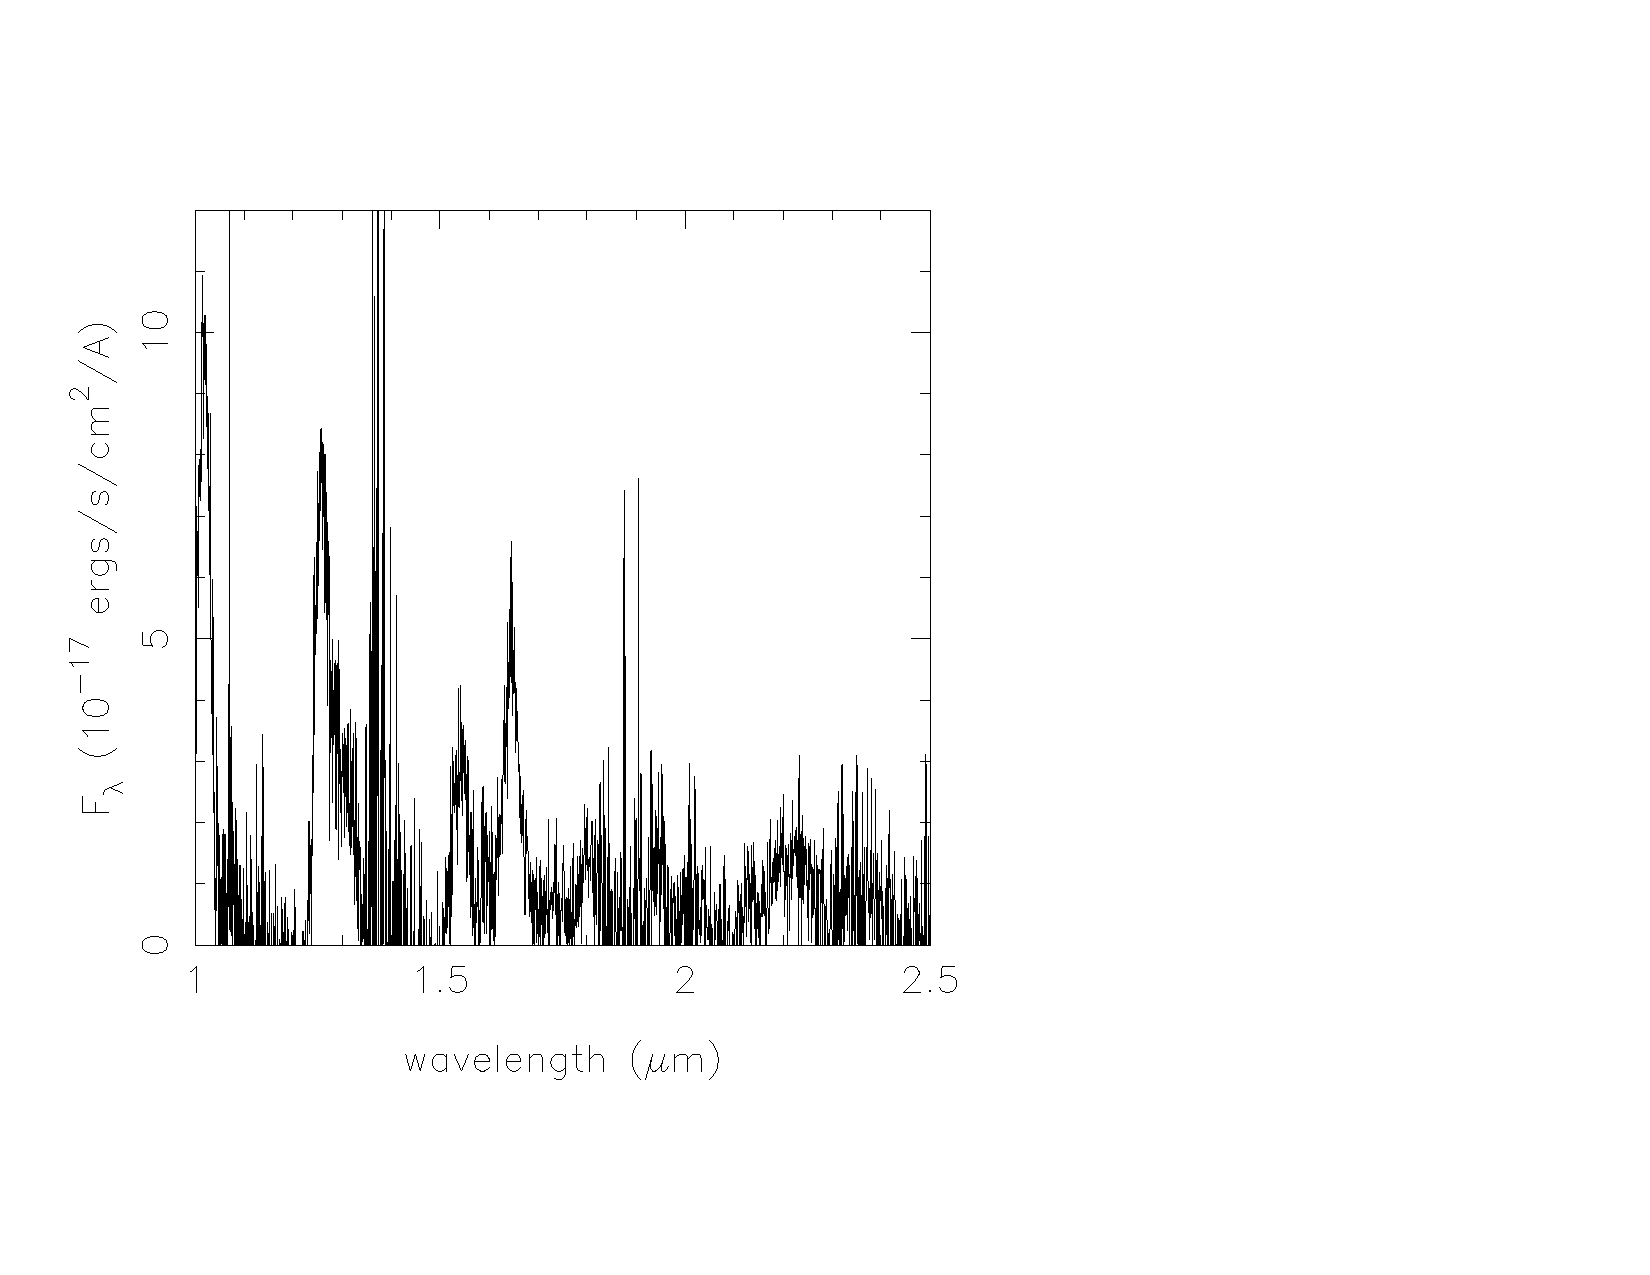
\includegraphics[width=.8\textwidth]{../0570fig1.pdf}
\caption{The NIR spectrum at +250 days for SN1998bu is shown from S04. We aim to improve upon the signal to noise and to observe the SN at later epochs. }%The figure shows the spectral energy distribution from the B to the K band for SN2014J (Johannsson et al. [2014]). The spectra are at phases of , +5d,+31d, +126d}
\end{figure}

%%%%%%%%%%%%%%%%%%%%%%%%%%%%%%%%%%%%%%%%%%%%%%%%%%%%%%%%%%%%%%%%%%%%%

% EXPERIMENTAL DESIGN
%
% THE EXPERIMENTAL DESIGN IS LIMITED TO ONE PAGE WITH 
% NO ADDITIONAL FIGURES.  Describe your overall observational program.  
% How will these observations contribute toward the accomplishment of the goals 
% outlined in the science justification?  Include information such as why the specific 
% targets were selected, the sample size, the analysis, etc.  Describe any necessary
% calibrations in addition to the baseline calibrations.

\expdesign    % Do not delete this command.

We propose to obtain 3 NIR spectra from the months of March to May. This will allow us to have  a time series of spectra between $\sim$ + 400 and $\sim$ +500 days. A time series at these epochs will allow us to clearly discern whether there is any evolution in the line velocities at late epochs. 
Having 3 spectra will allow us to look at the line velocity evolution in the SN. 

SN2014J is the nearest SNIa in close to 4 decades. Due to its brightness it offers a great opportunity to obtain high S/N late time observations which are not possible for other, more distant SNIa.

In order to study the late time properties of SN2014J, we have also proposed for photometric observations in the optical and NIR on the Himalayan Chandra Telescope (HCT). This will allow us to get a late time (pseudo)-bolometric light curve which can elucidate the configuration of the magnetic field in the ejecta. We will also we able to observe and time sample the late NIR light curve to understand the flattening in the JHK bands. 
%%%%%%%%%%%%%%%%%%%%%%%%%%%%%%%%%%%%%%%%%%%%%%%%%%%%%%%%%%%%%%%%%%%%%

% TECHNICAL CASE
%
% THE TECHNICAL CASE IS LIMITED TO ONE PAGE WITH NO
% ADDITIONAL FIGURES.  Also justify the instrument configuration, the exposure times 
% and the constraints requested (seeing, cloud cover, sky brightness and 
% if appropriate water vapor and elevation).  
% Specify the total time needed (including overheads), and the minimum requested 
% time. If you are applying for instruments on both Gemini North and Gemini South,
% please state the time request for each site.

\technicaldescription    % Do not delete this command.
We would like 15 exposures of 120 seconds  each per night. A total on source exposure time of 30 mins gives us an S/N of $\sim$ 50 (see ITC pdf attached ). For each such set of  exposures, the acquisition time is 12 mins. 
Hence, in total we request for 1 hour for each night (using a conservative estimate for overheads), and a total of 3 hours for the period of March to May. 

We would like to use the cross-dispersed mode in order to obtain a complete spectrum from 0.8 to 2.5 $\mu$m. Recently published observations of SN2005df (Diamond et al. [2014]) using GNIRS have also used cross-dispersion mode to get a complete spectrum from 0.8-2.4 $\mu$m.

The observations can be carried out during any phase of the moon. We would like to request clear nights for the observations. Details of the ITC are attached. 
\bigskip

%%%%%%%%%%%%%%%%%%%%%%%%%%%%%%%%%%%%%%%%%%%%%%%%%%%%%%%%%%%%%%%%%%%%%

% BAND 3 INFORMATION
% There is a limit of half a page of printed text.
% If you are applying for queue time, your ranking may place the program in 
% Band 3.  Band 3 observations are used to fill the queue when no Band 1 or 2 
% programs are available.  Successful Band 3 programs generally use poorer than 
% median observing conditions, have targets away from the most popular 
% regions of the sky, do not require strict timing or other constraints, 
% and do not require special instrument configurations.  Describe the changes
% you will make to the program to allow it to be successful in Band 3 in
% the \bandthreeplan section, or write "This program is not suitable for band 3"  
% or "This is not a queue request".  If a Band 3 allocation is acceptable and 
% the total Band 3 time request is different from the standard request, then 
% give the Band 3 time request for each partner and update the time requested
%  from each site.

\bandthreeplan    % Do not delete this command.


\bigskip

%%%%%%%%%%%%%%%%%%%%%%%%%%%%%%%%%%%%%%%%%%%%%%%%%%%%%%%%%%%%%%%%%%%%%

% CLASSICAL PROGRAM INFORMATION
% There is a limit of half a page of printed text.
% If you are applying for classical time on Gemini, please 
% define a backup program in case the weather is worse than
% the observing conditions in the proposal.  Enter your classical backup 
% in the \classicalbackup section, or write "The program as specified is 
% suitable for poor conditions, or "This is not a classical request".

\classicalbackup    % Do not delete this command.


\bigskip

%%%%%%%%%%%%%%%%%%%%%%%%%%%%%%%%%%%%%%%%%%%%%%%%%%%%%%%%%%%%%%%%%%%%%

% DUPLICATE OBSERVATIONS
% A search of the Gemini Science Archive 
% (http://www1.cadc-ccda.hia-iha.nrc-cnrc.gc.ca/gsa/) will reveal whether
% Gemini has previously been used to observe your targets using similar or
% identical observing setups.  If there are duplicate observations, please
% justify why new observations should be taken in the \justifyduplications
% section.  If the Archive search finds no duplicates, please enter
% ``The GSA search revealed no duplicate observations''.

\justifyduplications


\bigskip

%%%%%%%%%%%%%%%%%%%%%%%%%%%%%%%%%%%%%%%%%%%%%%%%%%%%%%%%%%%%%%%%%%%%

%  PUBLICATIONS
% 
% Enter a list of publications written by the PI and Co-Is that support 
% the current application. Use standard tex such as for the References section.

\publications          % Do not delete this command.
\begin{thebibliography}{99}
\bibitem[\protect\citeauthoryear{Taubenberger et 
al.}{2015}]{T15} Taubenberger S., et al., 2015, MNRAS, 448, 
L48 

\bibitem[\protect\citeauthoryear{Kerzendorf et 
al.}{2014}]{K14} Kerzendorf W.~E., Taubenberger S., 
Seitenzahl I.~R., Ruiter A.~J., 2014, ApJ, 796, LL26

\bibitem[\protect\citeauthoryear{Maguire et 
al.}{2014}]{KM14} Maguire K., et al., 2014, MNRAS, 444, 3258
\end{thebibliography}
\bigskip

%%%%%%%%%%%%%%%%%%%%%%%%%%%%%%%%%%%%%%%%%%%%%%%%%%%%%%%%%%%%%%%%%%%%


% OTHER FACILITIES AND PAST GEMINI USE
%

% List any applications to non-Gemini facilities that are related to this proposal.
% For each of these other facilities, indicate the nature
% of the observations (yours or those of others), and describe the
% importance of the observations proposed here in the context of the
% entire program. Or write: "There are no non-Gemini related proposals".

\otherfacilities    % Do not delete this command.


\bigskip

% List in the Table below allocations of Gemini telescope time  to the 
% Principal Investigator during the past 2 years (e.g. GN-2011A-Q-999), 
% the amount of time awarded (e.g. 12 hrs), 
% the percentage of this that was useful (e.g. 80), 
% and text describing the current state of any data obtained (e.g. Data reduced).  

\thepast    % Do not delete this command.


\begin{table}[h]
\begin{center}
\begin{tabular}{llcl}
Reference & Allocation & \% Useful & Status of previous data \\
\hline
 &  &  & \\
\hline
\end{tabular}
\end{center}
\end{table}

\bigskip

%%%%%%%%%%%%%%%%%%%%%%%%%%%%%%%%%%%%%%%%%%%%%%%%%%%%%%%%%%%%%%%%%%%%%%%%%%%


% ITC Attachments
%

% Use the Gemini Integration Time Calculator (ITC) for a typical source for each 
% instrument requested, see
% http://www.gemini.edu/sciops/instruments/integration-time-calculators
% Save the ITC output as a PDF file and include that in this section. The ITC pages 
% will not count against the page limits.  You may either merge the ITC PDF output 
% to the PDF version of this document or include the ITC PDF output
% using \includepdf, eg.
%
% \includepdf[pages={-}]{ITCoutput.pdf}
%
% See the PIT FAQ (http://www.gemini.edu/node/11087/) for additional suggestions.

\itcresults

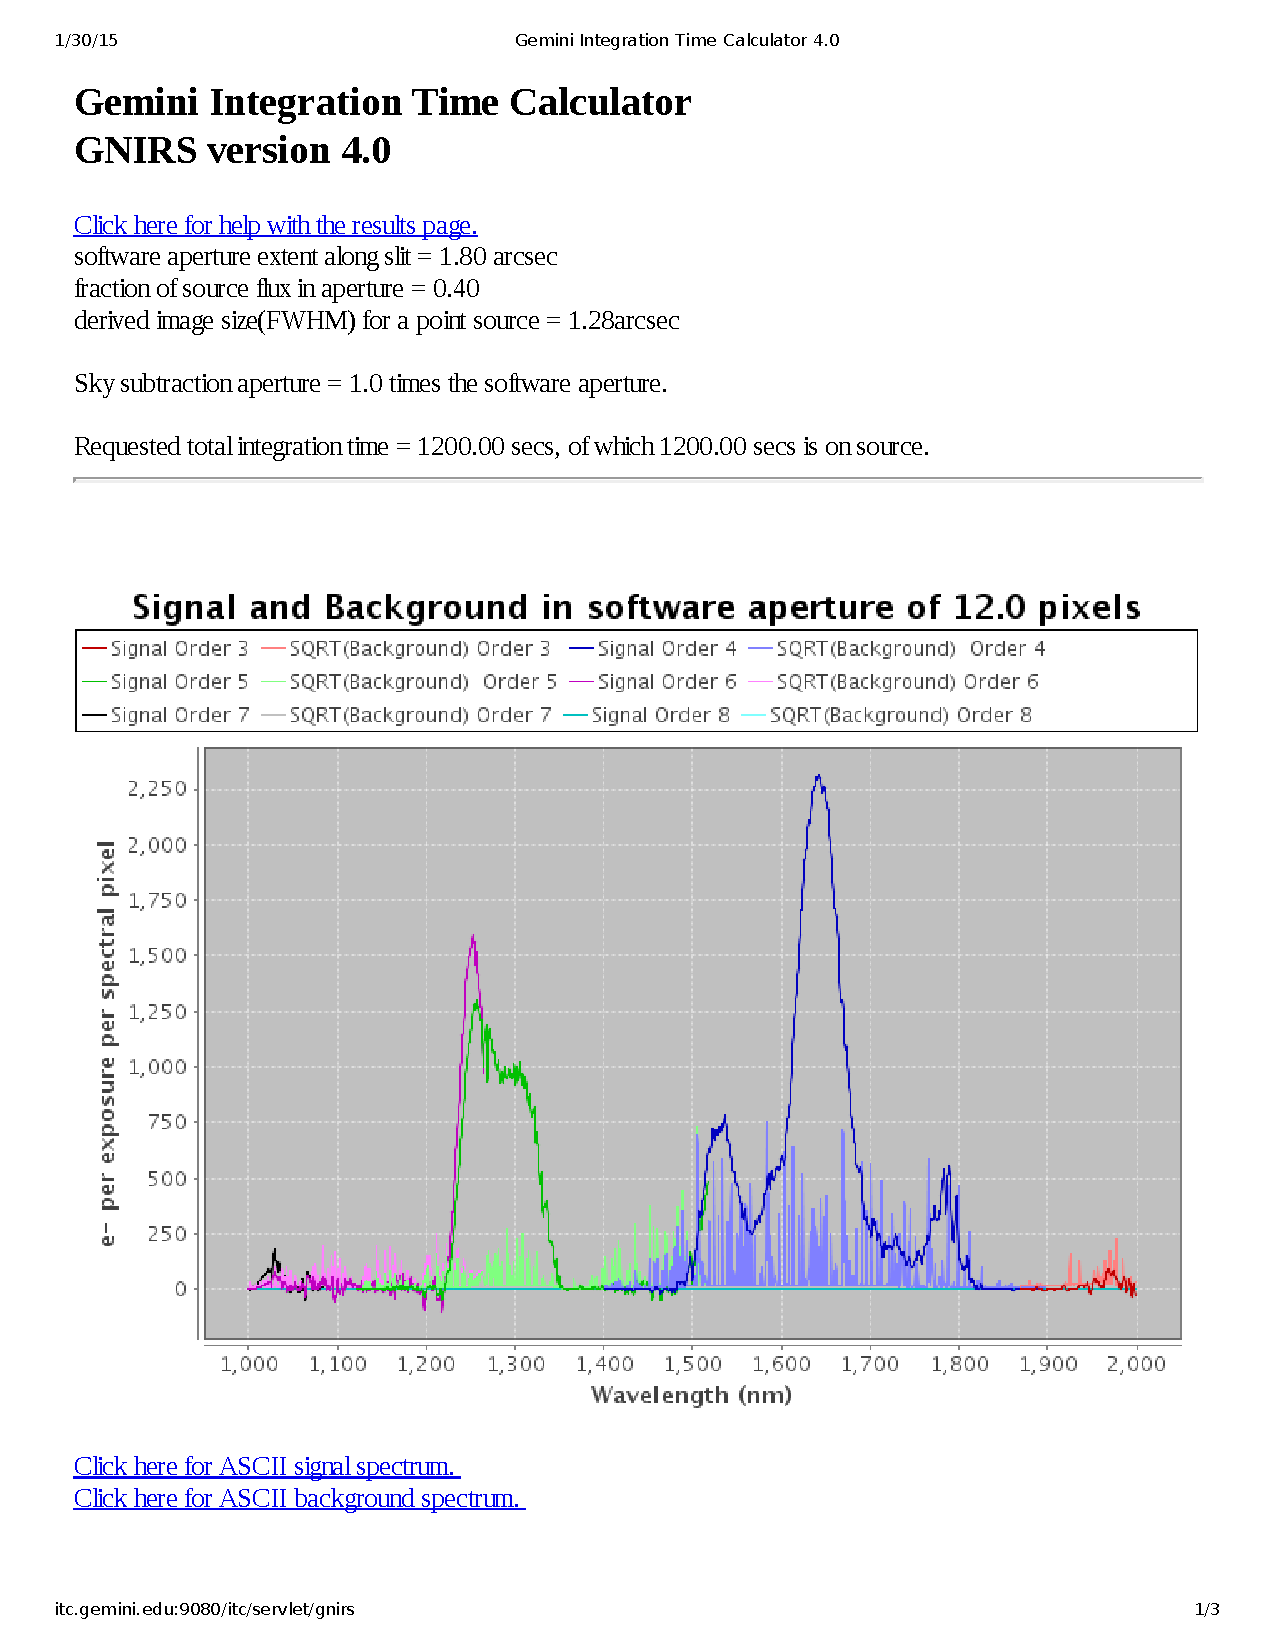
\includepdf[pages={-}]{../itc_14j.pdf}



%%%%%%%%%%%%%%%%%%%%%%%%%%%%%%%%%%%%%%%%%%%%%%%%%%%%%%%%%%%%%%%%%%%%%

% Please do not modify or delete this line.
\end{document}
